% Uncomment this to make slides with overlays:
%\documentclass[slides]{beamer}

% Uncomment these (but comment the above \documentclass line) to make handouts:
\documentclass[handout]{beamer}

% Uncomment these to have more than one slide per page
%\usepackage{pgfpages}
%\pgfpagesuselayout{2 on 1}[border shrink=5mm]
%\pgfpageslogicalpageoptions{1}{border code=\pgfusepath{stroke}}
%\pgfpageslogicalpageoptions{2}{border code=\pgfusepath{stroke}}

\usepackage[]{graphicx, color, hyperref}

\mode<presentation>
{
	%\usetheme[secheader]{Boadilla}
	%\usecolortheme[rgb={.835, .102,.169}]{structure}  
	\usetheme[width= 0cm]{Goettingen}
	%\setbeamercovered{transparent}
}
\setbeamertemplate{navigation symbols}{}
\setbeamertemplate{footline}[frame number]

\definecolor{blue2}{rgb}{0.278,0.278,0.729} 
\newcommand{\blue}[1]{\textcolor{blue2}{#1}}
\newcommand{\white}[1]{\textcolor{white}{#1}}
\newcommand{\red}[1]{\textcolor{red}{#1}}
\newcommand{\xbar}{\overline{x}}
\newcommand{\ybar}{\overline{y}}
\newcommand{\phat}{\widehat{p}}
\newcommand{\prob}{\mbox{Pr}}
\newcommand{\E}{\mathbb{E}}
\newcommand{\Var}{\mbox{Var}}
\newcommand{\cp}{\oplus}
\newcommand{\cm}{\circleddash}


\title{Lecture 26: Multiple Regression}
\author{Chapter 8.1}
\date{}


\begin{document}
%------------------------------------------------------------------------------
\begin{frame}
\titlepage
\end{frame}
%------------------------------------------------------------------------------


%------------------------------------------------------------------------------
\begin{frame}[fragile]
\frametitle{Categorical Predictor $x$ With Two Levels}

\begin{center}
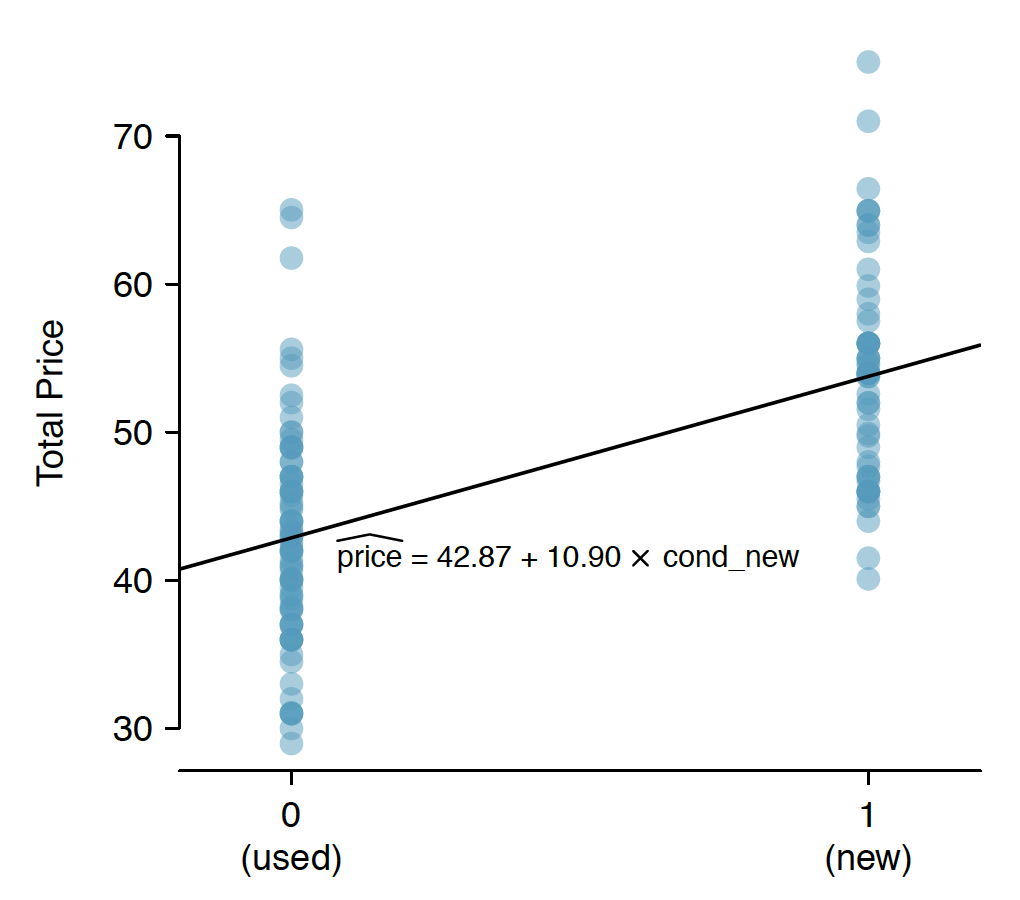
\includegraphics[width=0.75\textwidth]{figure/mario_kart.png}
\end{center}

\end{frame}
%------------------------------------------------------------------------------


%------------------------------------------------------------------------------
\begin{frame}[fragile]
\frametitle{Questions for Today}


Say on top of {\tt cond\_new} we are given three additional predictors:
\begin{center}

\includegraphics[height=3cm]{figure/mario_kart_action.png}
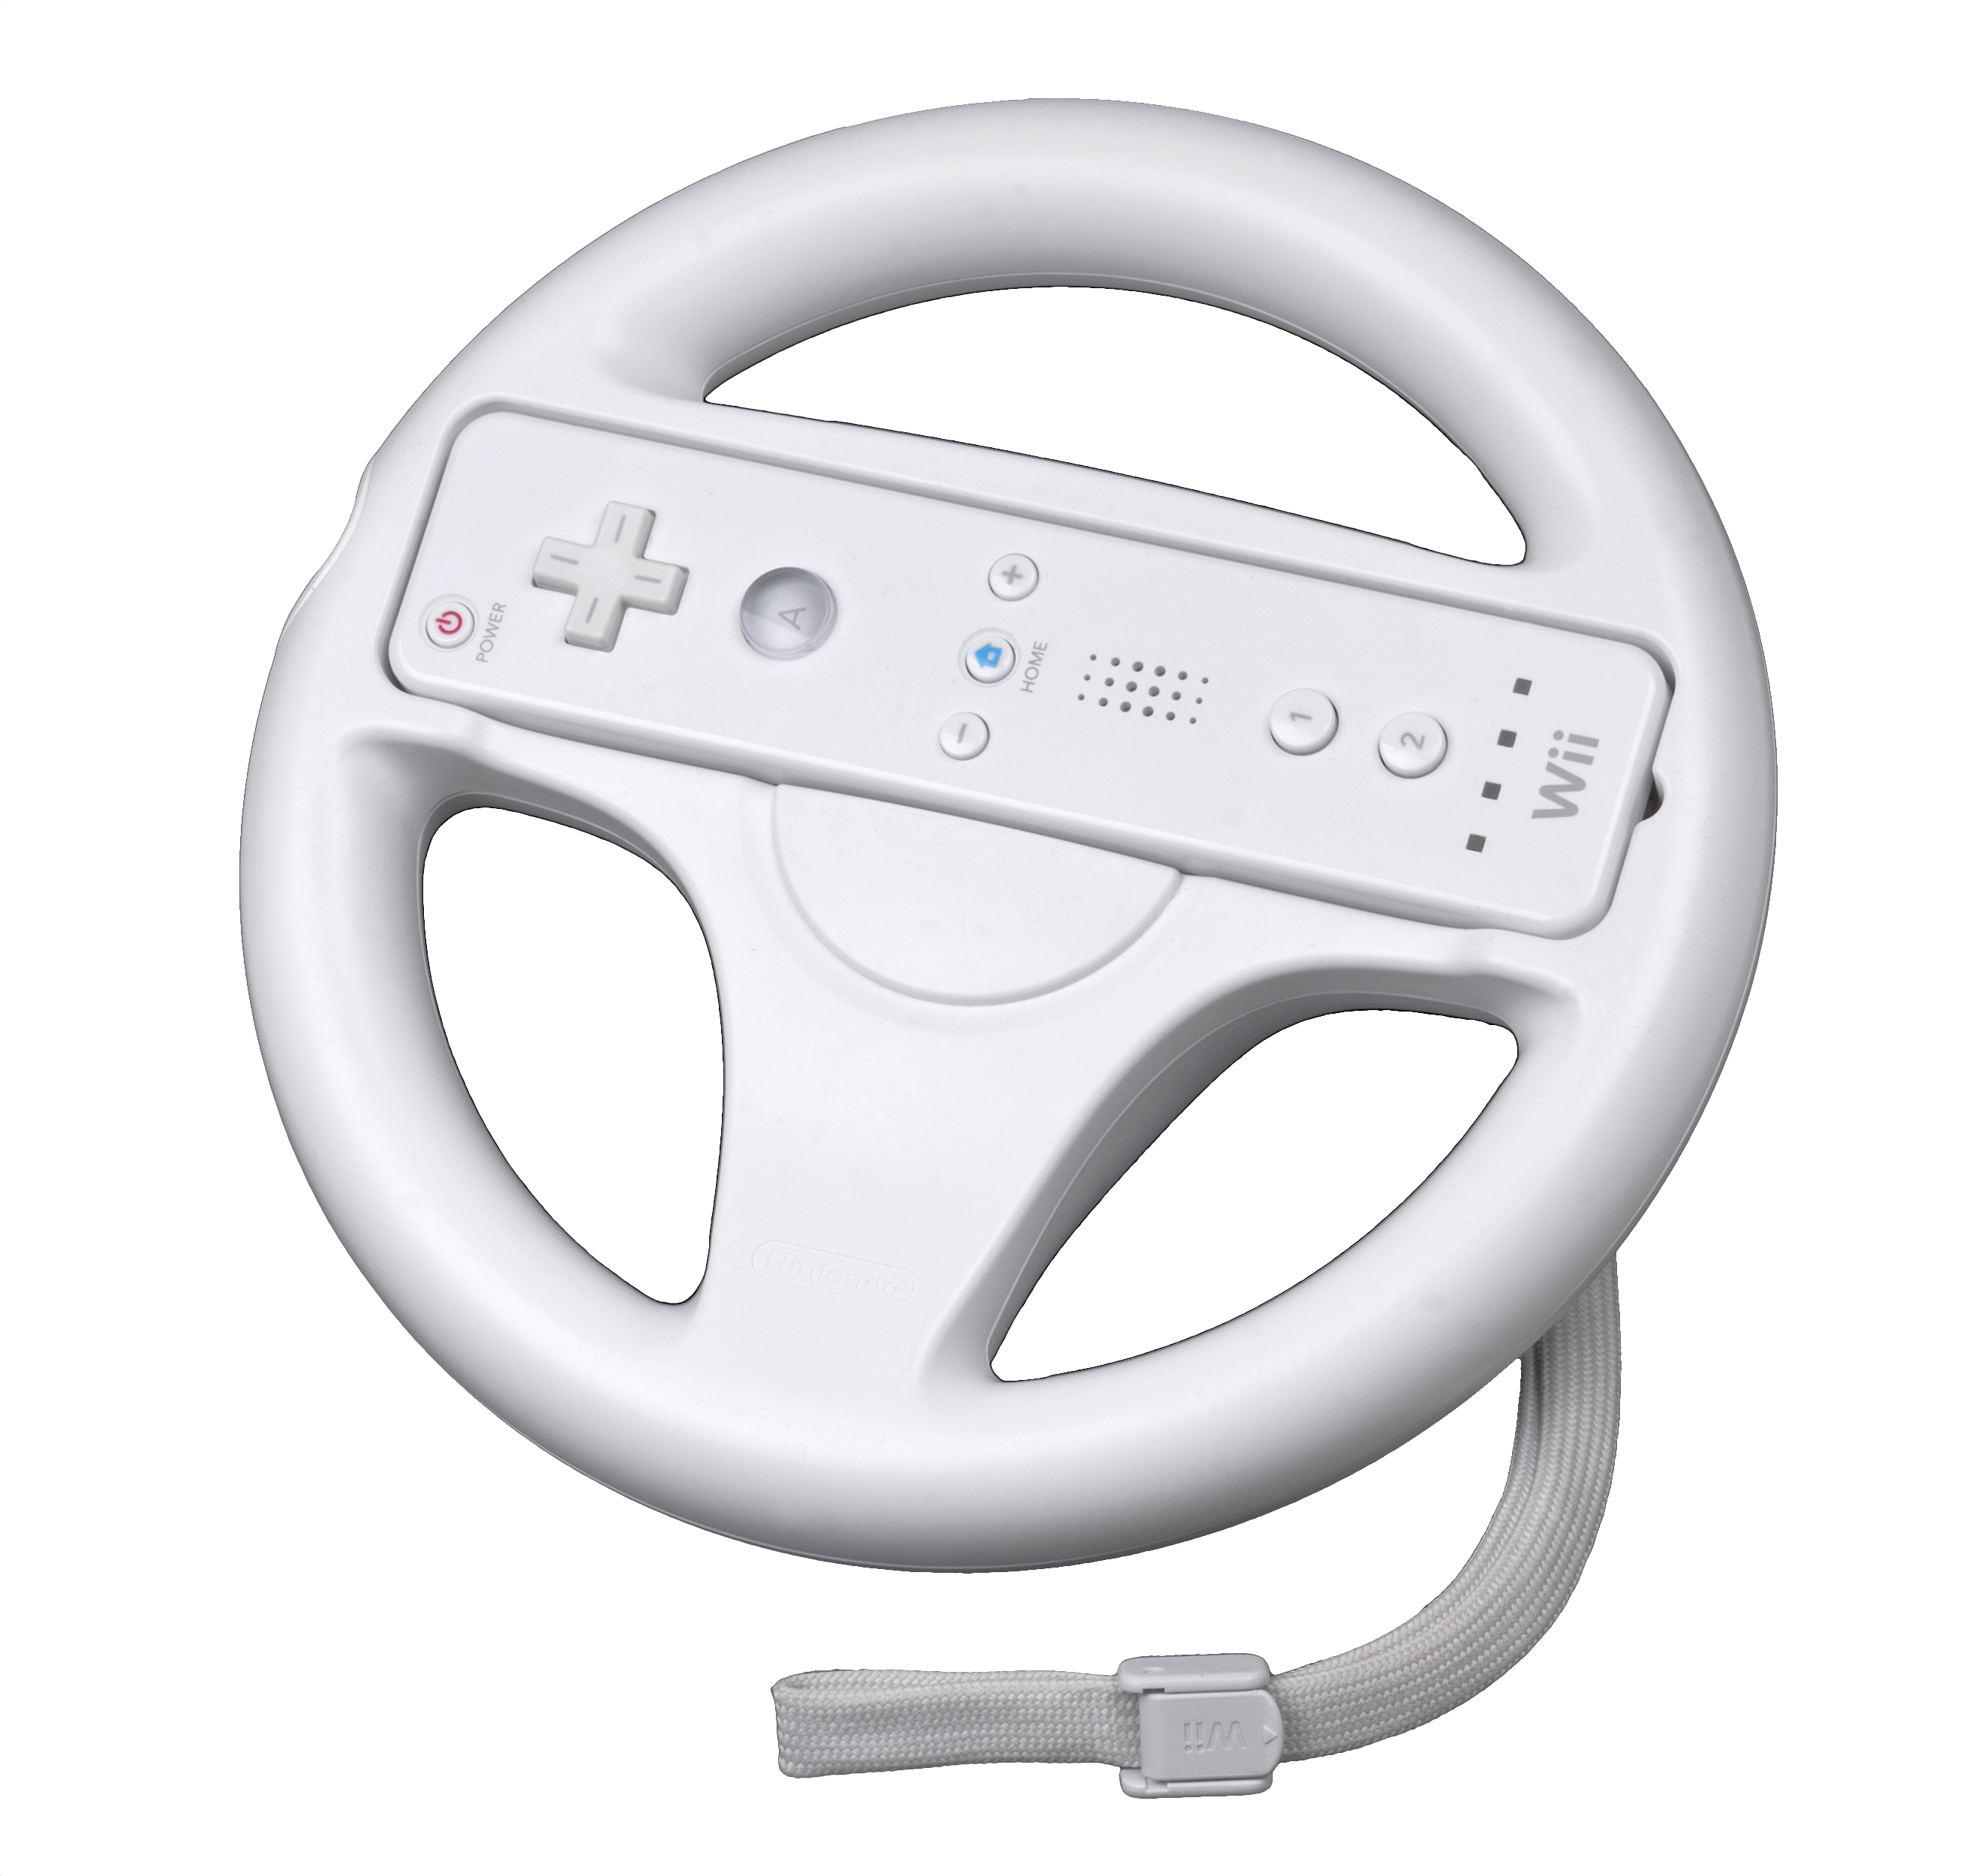
\includegraphics[height=3cm]{figure/wheel.png}
\end{center}
\pause

\begin{itemize}
\item {\tt stock\_photo}: is there a stock photo?
\item {\tt duration}: length of the auction in days (1 to 10)
\item {\tt wheels}: number of Wii wheels included
\end{itemize}


\end{frame}
%------------------------------------------------------------------------------


%------------------------------------------------------------------------------
\begin{frame}[fragile]
\frametitle{Questions for Today}

How do we simultaneously incorporate all four predictors to model the eBay auction {\tt price}?

\end{frame}
%------------------------------------------------------------------------------


%------------------------------------------------------------------------------
\begin{frame}[fragile]
\frametitle{Multiple Regression}
%
% Comment this
%
Use \blue{multiple regression} (done via computer) where
\begin{eqnarray*}
{\tt price} &=& \beta_0 + \beta_1 \times {\tt cond\_new} + \beta_2 \times {\tt stock\_photo} + \\ 
&&\beta_3 \times {\tt duration} + \beta_4 \times {\tt wheels}\\
\pause
\mbox{or in general...} &&\\
y &=& \beta_0 + \beta_1 x_1 + \beta_2 x_2 + \ldots + \beta_k x_k
\end{eqnarray*}
for $k$ predictor variables.

\end{frame}
%------------------------------------------------------------------------------


%------------------------------------------------------------------------------
\begin{frame}[fragile]
\frametitle{Point Estimates, Fitted Values, and Residuals}
%
% Comment this
%
Just as with SLR, we compute \blue{point estimates} $b_0, b_1, \ldots, b_k$ of the \blue{parameters} $\beta_0, \beta_1, \ldots, \beta_k$.

\pause\vspace{0.5cm}

For each observation $i=1,\ldots,n$ the $i^{th}$ \blue{residual} $e_i=y_i - \widehat{y}_i$.  The point estimates minimize the \blue{least squares criterion}:
\begin{eqnarray*}
\sum_{i=1}^{n} e_i^2 = \sum_{i=1}^{n} (y_i - \widehat{y}_i)^2
\end{eqnarray*}

\end{frame}
%------------------------------------------------------------------------------


%------------------------------------------------------------------------------
\begin{frame}[fragile]
\frametitle{Multiple Regression Results Table}

On page 357:
\begin{table}[ht]
\centering
\begin{tabular}{r|rrrr}
  \hline
 & Estimate & Std. Error & t value & Pr($>$$|$t$|$) \\ 
  \hline
(Intercept) & 36.21 & 1.51 & 23.92 & 0.00 \\ 
{\tt cond\_new} & 5.13 & 1.05 & 4.88 & 0.00 \\ 
{\tt stock\_photo} & 1.08 & 1.06 & 1.02 & 0.31 \\ 
{\tt duration} & -0.03 & 0.19 & -0.14 & 0.89 \\ 
{\tt wheels} & 7.29 & 0.55 & 13.13 & 0.00 \\ 
   \hline
   & & & & $df=136$\\
\end{tabular}
\end{table}
where $df=n-k-1=141-4-1=136$
\end{frame}
%------------------------------------------------------------------------------


%------------------------------------------------------------------------------
\begin{frame}[fragile]
\frametitle{Interpretation of Point Estimates}

%
% Comment this
%
The point estimates are interpreted as follows, for example:
\begin{itemize}
\item $b_4$ of {\tt wheels}:  \blue{holding all other variables constant} (\blue{all other things being equal}), the average difference in price associated with each additional Wii wheel is \$7.29.
\pause
\item $b_3$ of {\tt duration}:  \blue{holding all other variables constant}, every additional day of auction is associated with an average decrease of \$0.03 in price.  
\end{itemize}

\end{frame}
%------------------------------------------------------------------------------


%------------------------------------------------------------------------------
\begin{frame}[fragile]
\frametitle{Comparison of Results}

For simple linear regression:
\begin{table}[ht]
\centering
\begin{tabular}{r|rrrr}
  \hline
 & Estimate & Std. Error & t value & Pr($>$$|$t$|$) \\ 
  \hline
{\tt cond\_new} & 10.90 & 1.26 & 8.66 & 0.00 \\ 
   \hline
\end{tabular}
\end{table}
\pause
For multiple regression:
\begin{table}[ht]
\centering
\begin{tabular}{r|rrrr}
  \hline
 & Estimate & Std. Error & t value & Pr($>$$|$t$|$) \\ 
  \hline
{\tt cond\_new} & 5.13 & 1.05 & 4.88 & 0.00 \\ 
   \hline
\end{tabular}
\end{table}
Why the different point estimate?
\end{frame}
%------------------------------------------------------------------------------


%------------------------------------------------------------------------------
\begin{frame}[fragile]
\frametitle{Comparison of Result}

Because {\tt cond\_new} is linearly correlated with {\tt wheels}.  We say that two predictor variables are \blue{collinear} when they are correlated, and this complicates model estimation.

\pause\vspace{0.5cm}

In general we must be wary of predictor variables that are collinear, because the coefficient estimates may change erratically in response to small changes in the model or the data.

\end{frame}
%------------------------------------------------------------------------------


%------------------------------------------------------------------------------
\begin{frame}[fragile]
\frametitle{$R^2$ to Describe the Strength of Fit}
%
% Comment this
%
$R^2$ is a measure (between 0 and 1) of how well the model fits the data.  It measures the proportion of the total variability in $y$ explained by the model i.e. the least squares line:

\vspace{0.25cm}

\begin{eqnarray*}
R^2 &=& 1 - \frac{\mbox{variability in residuals}}{\mbox{variability in the outcome}}\\
&=& 1 - \frac{Var(e_i)}{Var(y_i)}
\end{eqnarray*}

\end{frame}
%------------------------------------------------------------------------------


%------------------------------------------------------------------------------
\begin{frame}[fragile]
\frametitle{Data Set Example 1}

\begin{center}
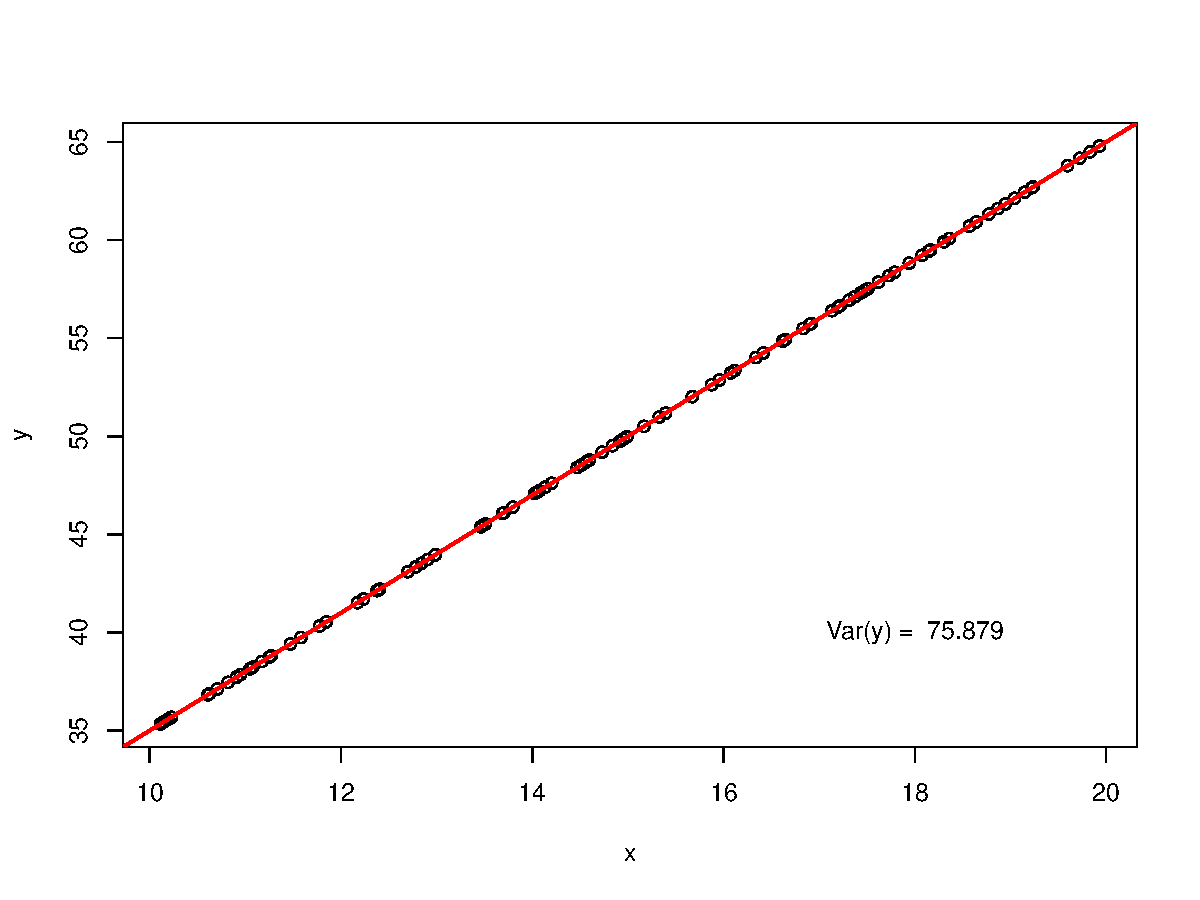
\includegraphics[width=\textwidth]{figure/plot1}
\end{center}

\end{frame}
%------------------------------------------------------------------------------


%------------------------------------------------------------------------------
\begin{frame}[fragile]
\frametitle{Data Set Example 1}

\begin{center}
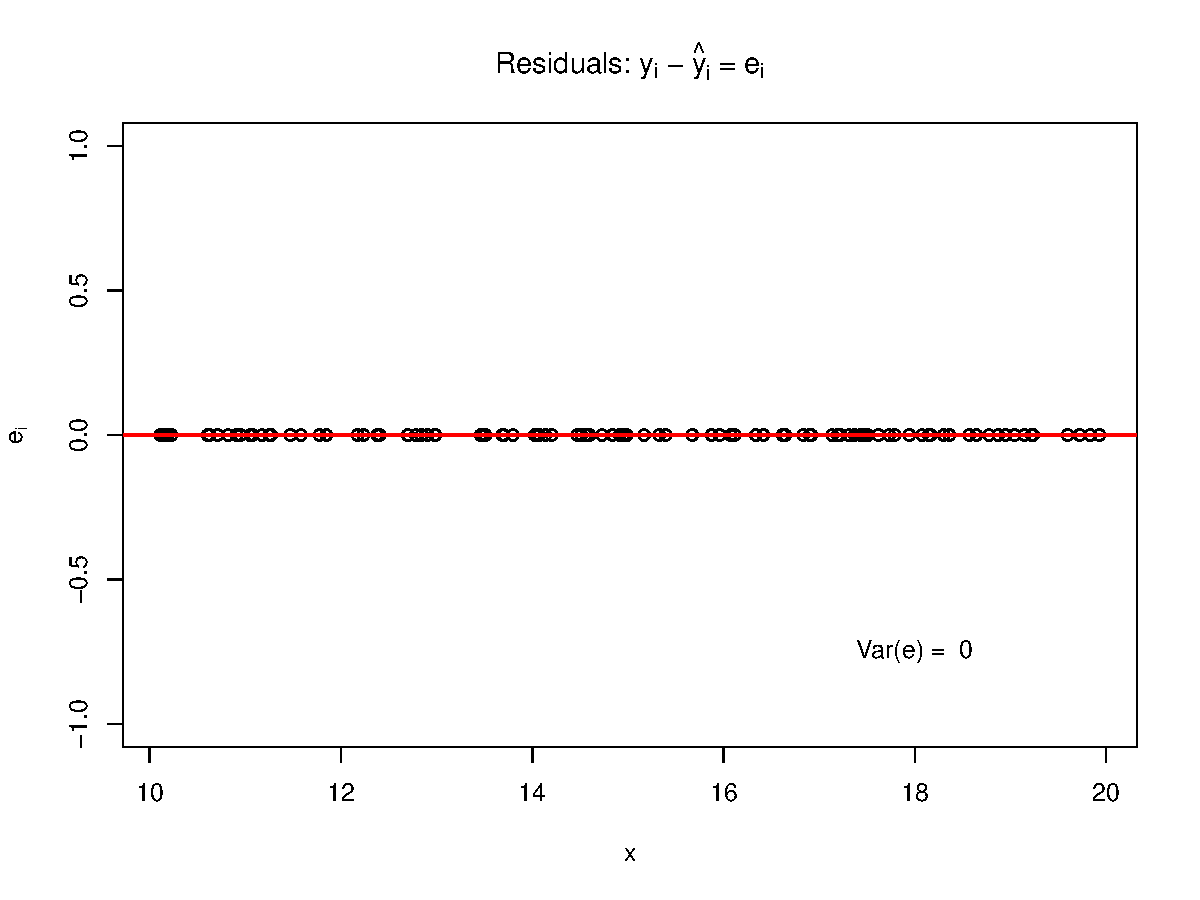
\includegraphics[width=\textwidth]{figure/plot2}
\end{center}

\end{frame}
%------------------------------------------------------------------------------


%------------------------------------------------------------------------------
\begin{frame}[fragile]
\frametitle{Data Set Example 2}

\begin{center}
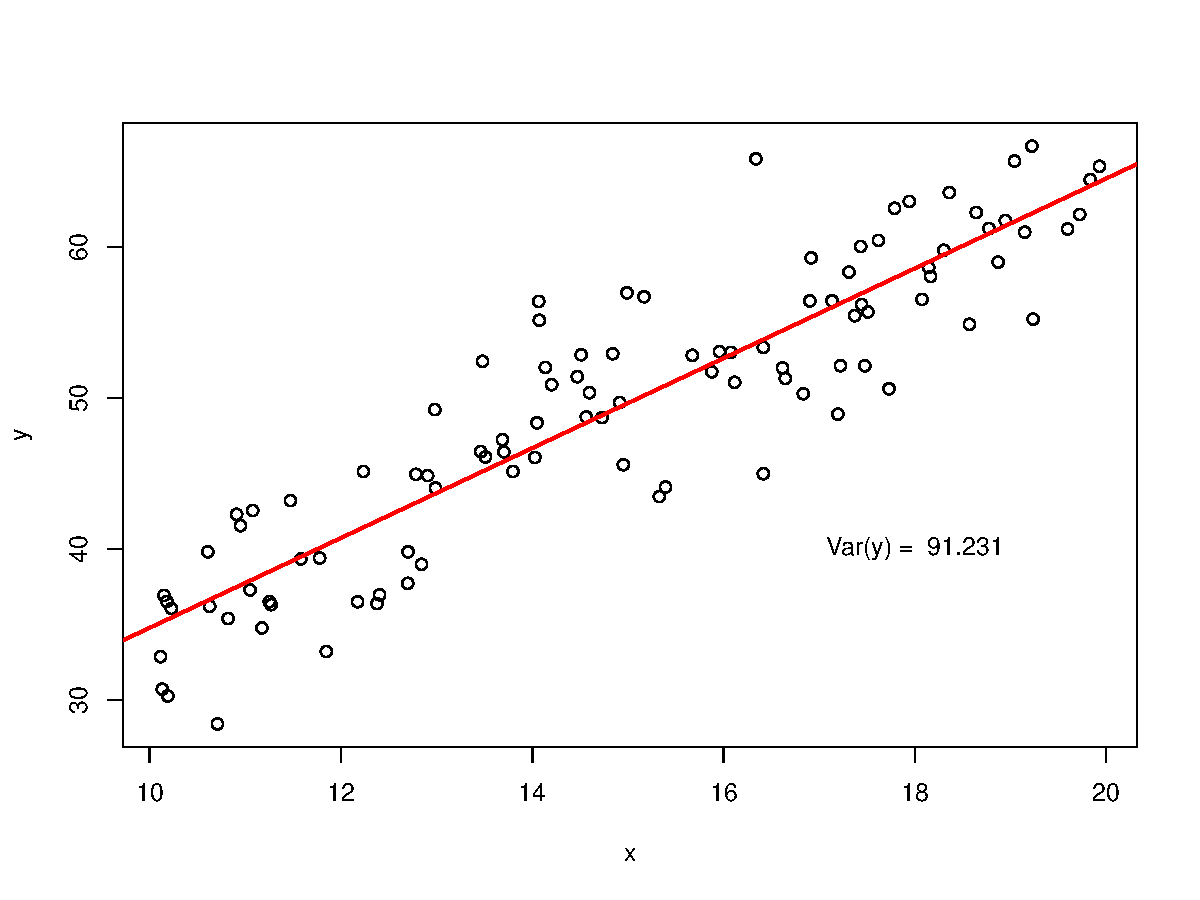
\includegraphics[width=\textwidth]{figure/plot3}
\end{center}

\end{frame}
%------------------------------------------------------------------------------


%------------------------------------------------------------------------------
\begin{frame}[fragile]
\frametitle{Data Set Example 2}

\begin{center}
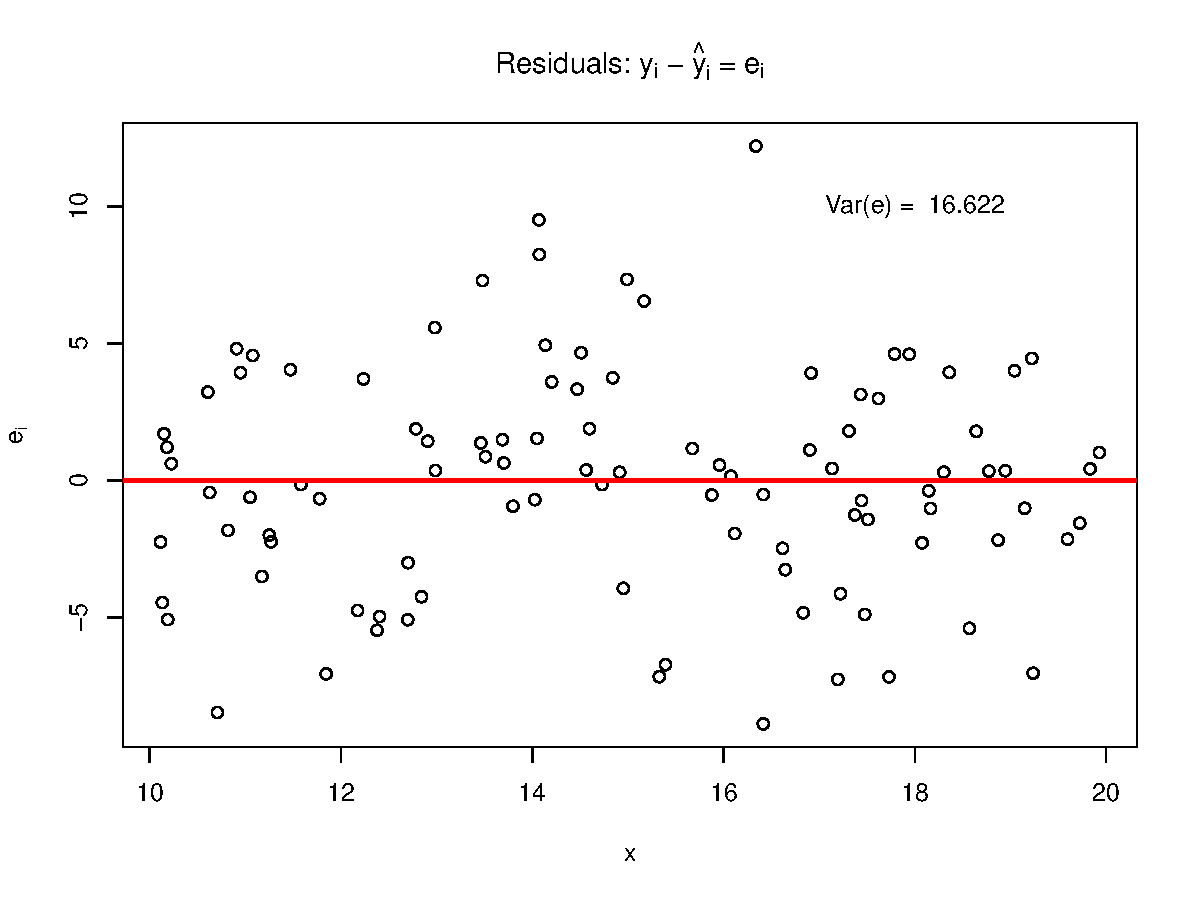
\includegraphics[width=\textwidth]{figure/plot4}
\end{center}

\end{frame}
%------------------------------------------------------------------------------


%------------------------------------------------------------------------------
\begin{frame}[fragile]
\frametitle{$R^2$ vs $R$}

Special case:  \blue{Only for linear regression}:  $R^2$ is the correlation coefficient $R$ squared.  The correlation coefficient \blue{does not exist} for multiple regression.  

\end{frame}
%------------------------------------------------------------------------------


%------------------------------------------------------------------------------
\begin{frame}[fragile]
\frametitle{Important Concept in Model Fitting}

$R^2_{adj}$ describes the strength of fit while adhering to the following:
\begin{itemize}
\pause\item \blue{Parsimony}:  Adoption of the simplest assumption in the formulation of a theory or in the interpretation of data.
\pause\item \blue{Occam's Razor}: When you have two competing theories that make exactly the same predictions, the simpler one is the better.
\end{itemize}


\end{frame}
%------------------------------------------------------------------------------


%------------------------------------------------------------------------------
\begin{frame}[fragile]
\frametitle{Adjusted $R^2_{adj}$}

%
% Comment this
%
The \blue{adjusted $R^2_{adj}$} takes into account the number of predictor variables $k$ you used to fit your model:  

\begin{eqnarray*}
R^2_{adj} = 1 - \frac{\frac{Var(e_i)}{n-k-1}}{\frac{Var(y_i)}{n-1}} = 1 - \frac{Var(e_i)}{Var(y_i)} \times \frac{n-1}{n-k-1}
\end{eqnarray*}

\end{frame}
%------------------------------------------------------------------------------


%%------------------------------------------------------------------------------
%\begin{frame}[fragile]
%\frametitle{Adjusted $R^2_{adj}$ as a Better Description of Fit}
%
%Note since 
%\begin{eqnarray*}
%R^2_{adj} &=& 1 - \frac{Var(e_i)}{Var(y_i)} \times \frac{n-1}{n-k-1}\\
%R^2 &=& 1 - \frac{Var(e_i)}{Var(y_i)}\\
%\pause\mbox{and } \frac{n-1}{n-k-1} &>& 1
%\end{eqnarray*}
%\pause
%in the case of $R^2_{adj}$ we are subtracting a bigger number, so for the same data we have
%\[
%R^2_{adj} > R^2
%\]
%\pause
%Furthermore, $R^2_{adj}$ can be negative.  
%
%\end{frame}
%%------------------------------------------------------------------------------


%------------------------------------------------------------------------------
\begin{frame}[fragile]
\frametitle{Parsimony/Occam's Razor}
%
% Comment this
%
Say for two models applied to the same data:
\begin{itemize}
\pause\item Model 1: $\widehat{y}_i = b_0 + b_1 x_{1,i}$ \ with residuals $e_i = y_i - \widehat{y}_i$
\pause\item Model 2: $\widehat{y}_i^* = b_0^* + b_1^* x_{1,i} + \blue{b_2^* x_{2,i}}$ \ with residuals $e_i^* = y_i - \widehat{y}_i^*$
\end{itemize}

\pause both models fit the data near identically, i.e. the residuals are similar
\begin{eqnarray*}
Var(e_i) \approx Var(e_i^{*}) \ldots
\end{eqnarray*}

\pause Then we should pick Model 1 over Model 2 since it is \blue{simpler}: it has fewer of predictors $k$.

\end{frame}
%------------------------------------------------------------------------------


%------------------------------------------------------------------------------
\begin{frame}[fragile]
\frametitle{Pared Down Mario Kart Regression Output}

\begin{small}
\begin{verbatim}
Coefficients:
              Estimate Std. Error t value Pr(>|t|)    
(Intercept)      41.34       1.71   24.15  < 2e-16
condused         -5.13       1.05   -4.88 2.91e-06
stockPhotoyes     1.08       1.06    1.02    0.308    
duration         -0.03       0.19   -0.14    0.888    
wheels            7.30       0.55   13.13  < 2e-16
---

Residual standard error: 4.901 on 136 degrees of freedom
Multiple R-squared:  0.719,	Adjusted R-squared:  0.7108 
\end{verbatim}
\end{small}

\pause Duration doesn't seem to be all that informative.  Why not drop it?

\end{frame}
%------------------------------------------------------------------------------


%------------------------------------------------------------------------------
\begin{frame}[fragile]
\frametitle{Pared Down Mario Kart Regression Output}

\begin{small}
\begin{verbatim}
Coefficients:
              Estimate Std. Error t value Pr(>|t|)    
(Intercept)      41.22       1.49   27.65  < 2e-16
condused         -5.18       1.00   -5.20 7.21e-07
stockPhotoyes     1.12       1.02    1.10    0.275    
wheels            7.30       0.54   13.40  < 2e-16
---

Residual standard error: 4.884 on 137 degrees of freedom
Multiple R-squared:  0.719,	Adjusted R-squared:  0.7128 
\end{verbatim}
\end{small}

\end{frame}
%------------------------------------------------------------------------------


%------------------------------------------------------------------------------
\begin{frame}[fragile]
\frametitle{Next Time}

Is there a systematic way to pick which predictor variables to include?

\pause\vspace{0.5cm}

Checking model assumptions as well.  

\end{frame}
%------------------------------------------------------------------------------


\end{document}

